\documentclass[12pt, letterpaper]{article}
\usepackage{
    graphicx,
    chemmacros,
    tikz,
    pgfplots,
    pgfplotstable,
    filecontents,
    datatool
}

\pgfplotsset{model/.style = {red}}


\title{Determination of the heat of hydration of bivalent copper sulphate pentahydrate}
\author{Afanasev S.M., Nesterov I.D.}
\date{}

\providecommand{\keywords} {
    \small	
    \textbf{\textit{Keywords:}}
} 

\begin{document}
    \maketitle
    \keywords{
        heat of formation,
        crystalline hydrate,
        copper sulphate}
    \tableofcontents
    \newpage

    \section{Introduction}
        \textbf{\textit{Purpose of work:}} to determine the heat of formation of crystalline hydrate \ch{CuSO4*}5\ch{H2O}. \\ 
        
        The heat of formation of crystalline hydrate \ch{CuSO4*}5\ch{H2O} will correspond to
        the reaction of addition of 5 moles of water to 1 mole of anhydrous salt according to the equation:

        \begin{equation}
            \ch{CuSO4\sld{}} + 5 {\ch{H2O}\lqd{}} = \ch{CuSO4*}5\ch{H2O\sld{},} \hspace{10 mm} \enthalpy*(hyd){}
        \end{equation}

        The thermal effect cannot be determined experimentally,
        because the formation of a new phase from liquid to solid phase is very slow and incomplete.
        Theoretical calculation of the thermal effect is carried out on the basis of Hess's law
        on the basis of the following cycle: 
        \begin{center}
        \begin{tikzpicture}
            \node (s) at (0,0) {\ch{CuSO4(solid)}};
            \node (aq) at (4,3) {\ch{CuSO4(solution)}};
            \node (h2o) at (8,0) {\ch{CuSO4 *} 5{H2O}};
            \draw[-latex] (s) -- node[above, rotate = 360]{$\overset{\enthalpy*(hyd) {}}{}$}(h2o);
            \draw[-latex] (h2o) -- node[above, rotate = -35]{$\overset{\enthalpy*(sol) {}\textsubscript{hyd}}{}$}(aq);
            \draw[-latex] (s) -- node[above, rotate = 35]{$\overset{\enthalpy*(sol) {}\textsubscript{dry}}{}$}(aq); 
        \end{tikzpicture}
        \end{center}
        
        where \enthalpy*(sol){}\textsubscript{dry} and \enthalpy*(sol){}\textsubscript{hyd} - integral heats of dissolution
        of anhydrous salt and crystalline hydrate, respectively. \\

        They are related by the following relationship:
        
        \begin{equation}
            \enthalpy*(hyd){} = \enthalpy*(sol){}\textsubscript{dry} - \enthalpy*(sol){}\textsubscript{hyd}    
        \end{equation}
        
        Also, the calorimeter constant must be determined before determining thermal effects. 
    \newpage
    \section{Methods and Results}
    \subsection{Determination of the calorimeter constant}
   
    For experimental determination of the calorimeter constant it is necessary to take a salt
    with a known heat of dissolution (for example: ammonium chloride).
    A beaker with 100 cm$^3$ of distilled water and a magnetic stirrer is placed in the calorimeter.
    For uniform heat distribution and complete dissolution of the salt, intensive stirring is carried out for 3-5 minutes (preparatory phase).
    After the preparatory phase, 2 grams of anhydrous salt is placed in the beaker (Main Period).
    The end of the "Main period" can be counted when the temperature begins to change linearly (at a constant rate).
    After another 10 counts are taken, this period will be considered the "end period". \\
     
    \begin{figure}[h]
        \centering
        \begin{tikzpicture}
            \begin{axis}[scale only axis,
                    width=10cm,
                    ylabel=$T$,
                    xlabel=$t$,
                    xmin=0, xmax=330,
                    ymin=21, ymax=23.2,
                    xtick={0,20,...,300},
                    xticklabel style={rotate=45, anchor=east},
                    ytick={21,21.2,...,23},
                    axis lines=middle,
                    grid=both
                ]
                \addplot[only marks] table [col sep=comma] {../data/raw/experiment1.csv};
                \addplot[model] table [col sep=comma] {../data/raw/experiment1.csv};

                \addplot[thick, smooth, magenta, color=black, dashed] coordinates {(100,22.434)(0,22.434)};
                \addplot[thick, smooth, magenta, color=black, dashed] coordinates {(170,21.269)(0,21.269)};
                \addplot[thick, smooth, magenta, color=black, dashed] coordinates {(0,21.8515)(220,21.8515)};    
                    \coordinate[label={90:$A$}] (A) at (axis cs:10,22.430);
                    \coordinate[label={90:$B$}] (B) at (axis cs:100,22.434);
                    \coordinate[label={90:$C$}] (C) at (axis cs:170,21.269);
                    \coordinate[label={90:$D$}] (D) at (axis cs:300,21.365);
                    \coordinate[label={90:$g$}] (g) at (axis cs:112.394,21.8515);
            \end{axis}
        \end{tikzpicture}
        \caption{Dissolution graph of \ch{NH4Cl} in distilled water}
    \end{figure}



        
     Determination of the calorimeter constant:
    \begin{equation}
       K = \frac{\Delta H_m \cdot m_{sal}}{ \Delta T \cdot M} - \left(m_{sal} - m_{water}\right) \cdot c 
    \end{equation}
        where $\Delta H_m$ - integral heat of dissolution of salt, expressed in J/mol;
        $\Delta T$ is the temperature change during experiment, measured in °C; 
        $m_{\text{sal}}$ and $m_{\text{water}}$ represent the mass of salt and water, respectively, in grams; 
        $M$ denotes the molecular weight of the salt, measured in g/mol; 
        and $c$ is the specific heat capacity of the resulting solution
        (the heat capacity of dilute solutions of inorganic salts in water is practically the same and slightly differs from the heat capacity of water, specifically $c = 4.184$ J/\ch{(g*K)}. \\ \\



        --a fucking place to calculate--

        \subsection{Determination of the heat effect of dissolution
anhydrous salt }
        For experimental determination of the heat effect of dissolution of anhydrous salt CuSO4. A beaker in which 100 cm³ of distilled water is poured and a magnetic stirrer is placed is placed in the calorimeter. For uniform heat distribution and complete dissolution of the salt, intensive stirring is carried out for 3-5 minutes (preparatory phase). After the preparatory phase, 2 grams of anhydrous salt is placed in the beaker (Main Period). The end of the Main Period can be determined when the temperature begins to change linearly (at a constant rate). Another 10 counts should then be taken and this period will be considered the "End Period".
        \begin{figure}[h]
            \centering
            \begin{tikzpicture}
                \begin{axis}[
                        ylabel=$T$,
                        xlabel=$t$,
                        xmin=0, xmax=330,
                        ymin=22, ymax=23.5,
                        xtick={0,20,...,300},
                        xticklabel style={rotate=45, anchor=east},
                        ytick={22,22.2,...,23.4},
                        axis lines=middle,
                        grid=both
                    ]
                    \addplot [only marks] table [col sep=comma] {../data/raw/experiment2.csv};
                    \addplot [model] table [col sep=comma] {../data/raw/experiment2.csv};
                        \coordinate[label={-90:$A$}] (A) at (axis cs:10,22.333);
                        \coordinate[label={-90:$B$}] (B) at (axis cs:100,22.368);
                        \coordinate[label={90:$C$}] (C) at (axis cs:140,23.323);
                        \coordinate[label={90:$D$}] (D) at (axis cs:300,23.324);
                \end{axis}
            \end{tikzpicture}
            \caption{Dissolution graph of \ch{CuSO4} in distilled water}
        \end{figure}
        Determination of the integral heat of dissolution of an anhydrous salt: 
        \begin{equation}
            \Delta_{sol}H^\circ_{dry} = \frac{(K + (m_{water} + m_{crystal}) \cdot c) \cdot \Delta T \cdot M_{crystal}}{m_{crystal}}
        \end{equation}
        where $ m_{crystal}$, $m_{water}$ - the mass of anhydrous salt and water, respectively, g; $M_{crystal}$ - is the molecular mass of anhydrous salt, g/mol; c - the specific heat capacity of the formed solution; $\Delta T$ - the temperature change during the experiment, °C. \\


        --a fucking place to calculate--
       


        \subsection{Determination of heat of dissolution of crystalline hydrate}
        As in experiment 2.2 all conditions remain the same, only instead of anhydrous salt the crystalline hydrate is used.
        \begin{figure}[h]
            \centering
            \begin{tikzpicture}
                \begin{axis}[
                        ylabel=$T$,
                        xlabel=$t$,
                        xmin=0, xmax=330,
                        ymin=22, ymax=22.2,
                        xtick={0,20,...,300},
                        xticklabel style={rotate=45, anchor=east},
                        ytick={22,22.02,...,22.2},
                        axis lines=middle,
                        grid=both
                    ]
                    \addplot [only marks] table [col sep=comma] {../data/raw/experiment3.csv};
                    \addplot [model] table [col sep=comma] {../data/raw/experiment3.csv};
                        \coordinate[label={-90:$A$}] (A) at (axis cs:10,22.038);
                        \coordinate[label={-90:$B$}] (B) at (axis cs:100,22.098);
                        \coordinate[label={90:$C$}] (C) at (axis cs:200,22.117);
                        \coordinate[label={90:$D$}] (D) at (axis cs:300,22.160);
                \end{axis}
            \end{tikzpicture}
             \caption{Dissolution graph of \ch{CuSO4*}5 \ch{H2O} in distilled water}
        \end{figure}
        Determination of the integral heat of dissolution of crystalline hydrate:
         \begin{equation}
            \Delta_{sol}H^\circ_{hyd} = \frac{(K + (m_{water} + m_{hyd}) \cdot c) \cdot \Delta T \cdot M_{hyd}}{m_{hyd}}
        \end{equation}
         where $ m_{hydl}$, $m_{water}$ - the mass of crystalline hydrate  and water, respectively, g; $M_{hyd}$ - is the molecular mass of crystalline hydrate, g/mol; c - the specific heat capacity of the formed solution; $\Delta T$ - the temperature change during the experiment, °C. \\

         --a fucking place to calculate--

         \subsection{Determination of the heat of formation of crystalline hydrate}
         The heat of formation of crystalline hydrate is calculated from Hess's Law by formula (2).
         \begin{equation}
            \enthalpy*(hyd){} = 
        \end{equation}

    \section{Conclusions}
        bla-bla-bla















    
    \newpage
    \section{References}
        1
        2
        3
        4

\end{document}